\documentclass[11pt,letterpaper]{article}
\usepackage[margin=0.85in]{geometry}
\usepackage[T1]{fontenc}
\usepackage[utf8]{inputenc}
\DeclareUnicodeCharacter{2212}{\ensuremath{-}}
\DeclareUnicodeCharacter{03B2}{\ensuremath{\beta}}
\DeclareUnicodeCharacter{2265}{\ensuremath{\geq}}
\DeclareUnicodeCharacter{2264}{\ensuremath{\leq}}
\DeclareUnicodeCharacter{2248}{\ensuremath{\approx}}
\DeclareUnicodeCharacter{0394}{\ensuremath{\Delta}}
\usepackage{lmodern,amsmath,amssymb,graphicx,tabularx,array,booktabs,float,hyperref}
\hypersetup{colorlinks=true,urlcolor=blue,pdfauthor={UCP Technology LLC},pdftitle={Detection imbalance shapes a transferred alpha cell reprogramming signature}}
\setlength{\parindent}{0pt}
\setlength{\parskip}{6pt}
\setlength{\emergencystretch}{3em}
\renewcommand{\arraystretch}{1.2}
\begin{document}
\begin{center}{\Large\bfseries Detection imbalance shapes a transferred alpha cell reprogramming signature}\par\vspace{8pt}UCP Technology LLC\par 27 October 2026\end{center}
\section*{Abstract}
Successful cell-state discrimination does not by itself establish the interpretation of a treatment contrast or the portability of a decision threshold. We examined a frozen 50-up/50-down alpha-cell reprogramming program in four drug-treated human islet donor preparations. Native reference AUROC was 0.859, but preparation detection at the strict source alpha-control threshold of zero was 48.5\%. An exact decomposition separated detected-feature imbalance from ranks among detected genes. Every positive native treatment contrast included reduced down-program detection; up-program detection also fell in two donors. These are arithmetic contributions, not evidence that the underlying biological change is purely technical. In independent Baron state and measurement controls, true thinning to 2,000 counts preserved donor mean alpha-versus-beta AUROCs of 0.992–0.999. The unchanged source threshold kept alpha false-positive fractions below 0.8\%, while beta-state detection fell by 6.2–11.7 percentage points on the same eligible cells. Holding each target donor’s negative native threshold fixed instead raised alpha positive fractions from 3.6–5.3\% to 12.9–20.9\%. A reusable diagnostic separates detection, rank components, eligibility and supplied-threshold decisions. The algebra applies to the stated score definition; the empirical findings concern the programs and datasets examined. Neither score movement nor mature-state classification establishes conversion.

\section*{Introduction}
Human alpha-cell reprogramming offers a possible source of insulin-producing cells, but an expression signature transferred between interventions measures resemblance before it measures source. PDX1/MAFA reprogramming and regenerative-drug exposure differ in perturbation, culture, and sampling [1,2]. A positive score in a current alpha-like population could reflect induction of an up-program, loss of a down-program, a change in sampled states, or technical capture. These possibilities require separate quantitative checks. The question here is how detection, positive-feature ranks, population selection, and score construction shape transport of one externally specified program.

Per-cell rank scoring is established through singscore, AUCell, and UCell [4–7], and detection-related bias has been benchmarked [8]. Our contribution connects an exact decomposition of this signed score to its treatment interpretation and to the consequences of transporting a fixed decision rule. We first assess native reference performance, then explain the primary treatment contrasts, test fixed decisions under count thinning in independent state controls, and examine gene-level contributions and limits. This separates useful ranking from score interpretation and threshold portability. Four donors provide four biological contrasts; neither cells nor repeated draws increase that number [9,10].

\section*{Data and analysis design}
GSE117454 supplied bulk alpha-GFP and alpha-PDX1/MAFA preparations for program construction [1]. Supplementary Table 8 verified four donor pairs: IIDP1697, IIDP1738, IIDP1770, and IIDP1776. GSE123844 supplied 158 alpha-control, 241 beta-control, 860 PM-preparation, and 77 graft-derived cells. A cell from a functionally successful PM preparation is not individually verified as converted. Single-cell donor identities are not mapped to barcodes; the graft material was author-flagged for limited quality and remains descriptive.

GSE266427 contains four donor islet preparations and four exposures per donor at 96 hours [2]. The main contrast is harmine 10 µM plus native GLP-1 5 nM versus DMSO. We use the eight relevant deposited integer-count matrices. All 16 deposited libraries contain 253,462 barcodes; numerical QC retains 177,149. QC requires at least 1,000 whole-library counts, 400 detected original feature rows, and mitochondrial fraction below 0.20. Duplicate symbols are summed after QC. The published final population has 109,881 cells; its curated barcode labels and identified corrected layer were not recovered by our source audit. This is an analysis of released counts, not exact replication of that population.

The original program and results were frozen before these subsequent analyses. Two internally frozen post-review plans specified decomposition, true thinning, population sensitivities, all five-program/three-scorer comparisons, fixed-threshold transport, gene contributions and matching rules before their respective new outputs were examined. Earlier findings, including Baron mean-score shifts, were already known. These plans are not public preregistration or an independent biological holdout. The supplementary gene-contribution subtraction was added after the third review had reported its expected outcome and is explicitly exploratory.

Each donor contrast is the treated minus vehicle mean cell score. We report donors separately; unequal captured-cell yields do not measure absolute tissue abundance. Technical draw variation is separate from biological uncertainty. Four donors, one duration and observational population selection do not support a cell-pooled biological significance test.

\section*{Frozen program, score, and operating points}
The candidate universe contains 12,051 genes shared across the reference and primary assay, excluding hormones, specified lineage/transgene markers, mitochondrial/ribosomal features, and cell-cycle genes. Candidate expression required CPM at least one in four bulk samples. Paired log2(CPM+1) changes selected 50 consistently positive and 50 consistently negative genes, ordered by median change with deterministic gene-name ties. Selection used only the four verified training pairs. The score subtracts mean fractional average rank in the down block from that in the up block; ranks include tied zeros. Hormone exclusions prevent direct insulin/glucagon readout but cannot remove all cell-state or capture dependence.

Native and simulated reference comparisons distinguish AUROC from detection at a chosen threshold. The threshold is the empirical alpha-control 95th percentile using linear interpolation and a strictly greater comparison; ties determine the achieved false-positive rate. The original simulations sampled empirical profiles and used multinomial draws at 2,000, 5,000, or 10,000 counts, including outside-universe mass. They may sample above observed depth and are observation-model simulations. They are kept separate from the new finite-library thinning experiments, which never create extra molecules. Preparation labels do not identify which individual cells truly converted.

\[s(x)=\frac{1}{m}\sum_{g\in U}\frac{r_g-1/2}{G}-\frac{1}{n}\sum_{g\in D}\frac{r_g-1/2}{G},\quad m=n=50,\ G=12051.\]
\section*{Exact decomposition and the common zero-rank baseline}
For nonnegative counts in a fixed universe and nonempty, disjoint up/down blocks, let K be the number of detected universe genes, kU and kD the detected up/down genes, and r+ the average rank among positive genes. With average tied-zero ranks, the score is exactly an occupancy term O plus a centered positive-rank remainder R. Neither term is a pathway or ancestry label. Integer half-rank arithmetic preserves exact mathematical zeros before floating conversion.

\[s=O+R,\qquad O=\frac{1}{2}\left(\frac{k_U}{m}-\frac{k_D}{n}\right)=\frac{k_U-k_D}{100}\quad(m=n=50).\]
\[R=\frac{1}{G}\left[\frac{\sum_{g\in U:x_g>0}(r_g^+-(K+1)/2)}{m}-\frac{\sum_{g\in D:x_g>0}(r_g^+-(K+1)/2)}{n}\right].\]
\[b=\frac{G-K}{2G},\qquad A_U=b+\frac{k_U}{2m}+R_U,\qquad A_D=-b-\frac{k_D}{2n}+R_D.\]
\section*{Component interpretation and fixed population membership}
Here AU and AD are the separately plotted signed block contributions, and RU+RD=R. The common baseline b rises when fewer universe genes are detected. Consequently, raw AU can increase while up-gene detection decreases. We make the occupancy terms primary and display zero-centered blocks AU−b and AD+b. The complete score is unchanged. The remainder obeys |R| ≤ (K−1)/(2G) times (kU/m+kD/n) for K≥1 and is zero at K=0; sparsity alone does not justify discarding it.

Broad alpha cells require GCG at least three counts and strict dominance over INS, SST, PPY, and GHRL. Strict alpha additionally requires GCG at least ten and detected ARX or IRX2. Cycle-high alpha uses the donor vehicle 75th percentile of positive cell-cycle fractions, held fixed across arms. These are expression proxies, not published cycling-alpha annotations or ancestry labels. Beta, mixed-endocrine, and other unassigned endocrine proxies provide additional population context; mixed cells can overlap alpha/beta selections.

True thinning draws d molecules without replacement from cells with observed whole-library counts N≥d, preserving outside-universe mass. Original population membership is fixed. Four depths (1,000, 2,000, 5,000 and 10,000) and five locked draws per depth are reported, always with native scores on those same eligible cells. A complementary sensitivity holds N≥10,000 membership fixed across depths using the existing draws. It isolates within-cohort depth response but selects a high-depth population. Counts remain available for small groups; displayed state fractions require at least 20 cells, and AUROC requires at least 20 of each state.

\section*{Decision transport and gene-level analysis}
For each original-program scorer, the native GSE123844 alpha-control q95 was saved before new target classifications and carried unchanged into all Baron donors and depths. The decision is strictly score>threshold. Separately, each Baron donor’s all-native alpha q95 was held fixed across depths. A third, explicitly recalibrated rule computes q95 on each depth-eligible alpha sample and evaluates it on those same cells: this is resubstitution, not held-out calibration. Its threshold is also applied unchanged to the fixed N≥10,000 subset. Original seeds and draw order reproduce the earlier thinning means; no additional biological replication is claimed.

For every selected gene and donor, signed occupancy contributions are +Δdetection/100 for up genes and −Δdetection/100 for down genes. Positive-rank contributions add to the retained score. Detection is reported separately from raw, CP10K and log1p(CP10K) means conditional on expression being positive; the latter compare different cross-sectional positive-cell sets. A shared top-ten-per-block display is ranked by equal-donor mean absolute occupancy contribution. All 100 genes, donor signs, absolute-contribution shares and concentration are retained.

A secondary specificity design sought 500 random programs with 50 genes per block, excluding the original genes. Vehicle-only matching was designed to preserve block detection and abundance asymmetry with locked per-slot calipers and per-donor/block balance checks. Fewer than ten candidate genes for any slot was a declared failure, without relaxed calipers or a partial-control percentile. The vehicle candidate lists and failure or accepted programs were frozen before any new-program treatment effects.

\section*{Native reference calibration already limits detection}
Native PM-versus-alpha AUROC was 0.859. However, the alpha q95 threshold was exactly zero: 417/860 PM-preparation cells exceeded it (48.49\%), while 3/158 alpha controls did so (1.90\%). Thus limited preparation detection precedes any artificial depth reduction. Changing the comparison to greater-than-or-equal would include zero ties and increase alpha false positives to 10.13\%; it is not the retained rule. Median whole-library counts were 16,026.5 for PM and 10,091 for alpha controls, with median detected signature genes 14 and nine, respectively.

Mean detected up/down block sizes were 1.47/9.04 in alpha controls, 7.17/6.97 in PM preparations, and 7.59/2.73 in beta controls. These empirical capture means expose an asymmetry that total detected-feature counts conceal: alpha cells primarily detect the down block, PM preparations are more balanced, and beta cells primarily detect the up block. They are descriptive averages over captured cells, not estimated conversion fractions.

The original multinomial simulations retained positive-preparation detection of 25.75\%, 30.50\%, and 42.50\% at increasing depths against alpha-only or pooled 0–10\% beta-RNA comparators. The frozen gate required both AUROC at least 0.80 against each declared comparator and preparation detection at least 0.80 at every tested depth. This 80\% detection threshold is an analyst-chosen use criterion, not a biological necessity or clinical standard. The detection requirement failed even without 20\%/50\% stress mixtures. These results limit a particular program and operating point; they neither erase its ranking information nor estimate true conversion sensitivity. Native beta controls and the low-quality graft preparation have different targets and are shown separately in Figure 1.

\section*{Positive donor shifts include loss of down-program detection}
Native broad-alpha contrasts were positive in all four donors, ranging from +0.00474 to +0.02451. Occupancy accounted arithmetically for +0.00523, +0.01242, +0.01735, and +0.01917 in D1–D4; the rank remainder opposed the D1 shift and reinforced the other three. Detected down-block genes declined in every donor. Detected up-block genes also declined in D2 and D4, by 0.42 and 0.68 genes per cell on average. A positive contrast therefore cannot be read simply as greater detection of the up-program. Table 1 reports the additive components without turning their ratios into causal attribution.

The raw up-rank plot would obscure this mechanism. In D4, mean detected universe genes fell by 940, raising b by 0.03900. Raw AU increased by 0.03298, but its zero-centered contribution fell by 0.00603. D2 showed the same sign discrepancy. Figure 3 displays occupancy and zero-centered blocks; Figure S1A shows the baseline-containing components.

Treated broad-alpha libraries had lower median whole-library counts in every donor. Within-sample depth associations and deciles are descriptive and can reflect biology, capture, and selection together. Population choice also matters: D1 changed from +0.00474 in broad alpha to +0.00138 in strict alpha and −0.01644 in the cycle-high proxy. The other cycle-high contrasts remained positive. This reversal identifies a population dependence; it does not refute the published cycling-alpha hypothesis because the proxies and deposited layer do not reproduce that curated target.

\begin{table}[H]\small
\textbf{Table 1. Broad-alpha contrasts. Native full-cohort score equals occupancy plus remainder. The last two columns use exactly the same N≥2,000 cells; thinning is mean ± technical SD over five draws.}\par\vspace{5pt}
\begin{tabularx}{\linewidth}{>{\raggedright\arraybackslash}X>{\raggedright\arraybackslash}X>{\raggedright\arraybackslash}X>{\raggedright\arraybackslash}X>{\raggedright\arraybackslash}X>{\raggedright\arraybackslash}X}
\toprule
\textbf{Donor} & \textbf{Native, full} & \textbf{Occupancy} & \textbf{Remainder} & \textbf{Native, same eligible} & \textbf{Thinned, 2,000 counts}\\\midrule
D1 & +0.00474 & +0.00523 & -0.00048 & +0.00899 & +0.00102 ± 0.00056\\
D2 & +0.01364 & +0.01242 & +0.00122 & +0.01285 & -0.00243 ± 0.00037\\
D3 & +0.02066 & +0.01735 & +0.00331 & +0.02341 & +0.00607 ± 0.00092\\
D4 & +0.02451 & +0.01917 & +0.00534 & +0.02445 & -0.00186 ± 0.00019\\
\bottomrule\end{tabularx}
\end{table}
\section*{True thinning separates molecule loss from cohort eligibility}
At 2,000 counts, mean broad-alpha contrasts were +0.00102, −0.00243, +0.00607, and −0.00186 for D1–D4. All five draws agreed in sign within each donor. The corresponding native contrasts on those same eligible cells were +0.00899, +0.01285, +0.02341, and +0.02445. This change describes the imposed thinning operation on captured molecules; it does not identify the cause of native treatment differences.

The full depth series prevents a selective low-depth conclusion. At 10,000 counts, D2 and D4 regained positive thinned contrasts, while D1 was negative and D3 remained positive. Only 419 of 4,938 treated D4 broad-alpha cells were eligible there, compared with 1,020 of 1,957 controls. In D1, the same-eligible native contrast was already negative at 5,000 and 10,000 counts. Thus both retained molecules and which cells remain eligible alter the observed result. Figure 3 displays native eligible-cohort comparators and counts at every depth, rather than treating thinning as an unbiased correction of treatment biology.

Holding N≥10,000 membership fixed gives a separate depth-response check (Figure S1B). D1 remains negative across all depths, D2 changes from negative to positive, and D3 remains positive. D4 is −0.00108 at 1,000 counts, +0.00064 at 2,000 and +0.01282 at 10,000; its 2,000-count technical SD is 0.00091. This differs from the depth-specific-eligible D4 mean of −0.00186 at 2,000. Cohort choice therefore changes the displayed response even when original masks are fixed; the high-depth subset is not an unbiased correction.

\section*{Independent state and measurement control}
The four original human Baron files contain 8,569 labeled cells, including 2,326 alpha and 2,525 beta cells [3]. Original cell identifiers are unique; bare barcodes repeat across libraries and were not merged. All counts are nonnegative integers. Of 12,051 universe genes, 11,694 are represented, including all 50 up genes and 49 down genes. Missing TMEM236 is zero-filled in the main original-universe analysis. An explicitly separate shared-feature reranking sensitivity updates the universe and block denominators without refitting.

The frozen original fractional-rank score strongly discriminated published beta from alpha states: donor AUROCs were 0.9947–0.9998. This positive control is incompatible with a claim that the score is generally uninformative. Log-expression also discriminated these states strongly; original UCell-form AUROCs were 0.9136–0.9567. At the same time, true thinning to 2,000 counts increased alpha scores by +0.02071 to +0.03399 and decreased beta scores by −0.02137 to −0.00830 on their respective eligible cells. Opposite changes are expected when sparse detection moves differently signed states toward zero. These are independent state and measurement controls, not conversion validation.

The independent labels were supplied by the original study, not assigned using this score. They remain transcriptomic cell-state annotations rather than permanent lineage or secretion measurements. No independent cells were used to refit genes or choose a preferred scoring method. The shared-feature sensitivity and all feature programs are retained so that missing-gene handling cannot be chosen retrospectively to improve apparent validation.

\section*{Strong state ranking does not ensure fixed-threshold portability}
At 2,000 counts, donor mean signed-rank AUROCs remained 0.9919–0.9987, yet the consequences for fixed decisions depended on the threshold (Figure 4; Table 2). All four source-defined scorer q95 thresholds were exactly zero. For signed ranks, alpha false-positive fractions after thinning were 0–0.76\%, despite increased mean alpha scores. Source-threshold beta-state detection fell from 85.8–93.0\% in the same eligible native cells to 74.1–84.9\%, a donor-specific loss of 6.2–11.7 percentage points. At 1,000 counts, alpha false-positive fractions were still 0.07–2.04\%, while beta-state detection was 60.2–73.0\%. Thus the source rule mainly lost beta-state detection while retaining low alpha-positive fractions.

A negative native target threshold behaved differently. Baron donor alpha q95 values ranged from −0.04158 to −0.02046. Holding each fixed at 2,000 counts raised alpha positive fractions to 12.9–20.9\%, from 3.6–5.3\% on those same eligible native cells. At 1,000 counts they reached 40.8–58.9\%. Recalibrating within each depth returned alpha rates close to the empirical target, subject to ties and finite sample size, but that result uses the evaluation cells themselves. Human3 at 1,000 counts had recalibrated q95=0 and 2.04\% achieved FPR. Recalibration cannot be read as independently validated specificity.

Ranking, score scale and decisions therefore have distinct stability properties. Thinned rates and AUROCs are donor means over five technical draws. Per-cell transitions, ties, all depths, all four scoring definitions and the selected fixed high-depth cohort are retained. At 10,000 counts, only human4 has at least 20 alpha and beta cells, limiting that ranking comparison. These are mature-state classification results; they do not estimate false-positive or false-negative conversion calls.

\begin{table}[H]\small
\textbf{Table 2. Original rank-score decisions at 2,000 counts. Each pair is native / thinned on the same eligible cells; thinned percentages average five draws. Source threshold stays zero. Target-native thresholds stay at each donor’s original negative alpha q95. Labels indicate cell state, not conversion.}\par\vspace{5pt}
\begin{tabularx}{\linewidth}{>{\raggedright\arraybackslash}X>{\raggedright\arraybackslash}X>{\raggedright\arraybackslash}X>{\raggedright\arraybackslash}X>{\raggedright\arraybackslash}X}
\toprule
\textbf{Donor} & \textbf{Eligible alpha / beta n} & \textbf{Source alpha FPR (\%)} & \textbf{Source beta detection (\%)} & \textbf{Fixed target alpha FPR (\%)}\\\midrule
human1 & 221 / 839 & 0.45 / 0.27 & 85.8 / 74.1 & 3.6 / 20.9\\
human2 & 639 / 355 & 0.16 / 0.16 & 93.0 / 84.9 & 4.1 / 17.1\\
human3 & 1081 / 758 & 0.46 / 0.76 & 88.9 / 82.7 & 4.4 / 12.9\\
human4 & 283 / 488 & 0.00 / 0.00 & 92.2 / 84.5 & 5.3 / 14.6\\
\bottomrule\end{tabularx}
\end{table}
\section*{A reusable measurement diagnostic}
The released diagnostic accepts an explicit gene universe, disjoint up/down blocks, a genes-by-cells count matrix, aligned cell metadata and optional threshold provenance. Its report separates up/down detection, occupancy, positive ranks, the zero baseline, eligible fractions and strict-threshold decisions. It flags a positive group contrast accompanied by lower up detection without labeling that flag as a failed biological experiment. A synthetic example and worked primary-D4 and Baron reports show how to inspect the mechanism and then ask whether the intended decision changes. The diagnostic proposes neither a corrected score nor an unvalidated universal pass/fail cutoff.

\section*{Mixed gene contributions and influence on the net contrast}
AGT and SMARCA1 were the two largest down-block contributors by equal-donor mean absolute occupancy change; reduced detection in each contributed positively in all four donors. Other leading genes opposed the shift: greater KLHL41 and LOXL4 detection contributed negatively in every donor. Among up genes, PLCXD2 and SLC4A8 lost detection in all four donors, although conditional-positive CP10K means rose in three donors for each. Thus detection and positive-expression changes are distinct, and the result is not a uniform change across one block (Figure 5).

The shared top ten account for 51.5\% of down-block and 62.2\% of up-block mean absolute occupancy change; within-block concentration indices were 0.038 and 0.051. Absolute concentration does not measure the stability of a small net signed contrast. In an exploratory subtraction of each gene’s complete zero-centered contribution, no single subtraction reversed any donor’s positive native contrast. Subtracting each donor’s five largest positive contributions reversed D1 and slightly reversed D2, while D3 and D4 remained positive (Appendix F; Table S1). These arithmetic influences use the original universe and denominators, without reranking or refitting.

The matched-random specificity comparison failed its locked support requirement before program sampling: SPINK1 and TM4SF4 had no eligible replacements, RSAD2 had two, PLCE1 four, and VIM nine. All were down-block slots. No programs or specificity percentiles were produced, and calipers were not widened. This unsuccessful control construction provides no evidence either that the program is unusually specific or that similarly sparse programs behave the same way. The algebra generalizes to the stated score definition; demonstrated empirical behavior remains bounded by the programs and datasets examined.

\section*{Feature stability does not remove scorer dependence}
Four leave-one-training-donor-out programs repeat the same selection rule on three pairs and the frozen universe. Their side-specific Jaccard overlap with the original ranged from 0.587 to 0.786. This measures training-feature stability, not unbiased held-out validation: the universe and analytical choices were already selected. Each of the five programs was evaluated with fractional ranks, signed mean log1p(counts-per-10,000), and a fixed UCell-form comparator. All 20 native rank contrasts were positive. D2 log-expression contrasts were negative for every program, from −0.03237 to −0.00771. D4 log-expression signs varied by program.

The UCell-form comparator uses capped descending ranks (1,500), the updated denominator, and a signed combination clipped at zero [7]. In the original program, 98.74–99.94\% of broad-alpha cells in the eight vehicle/treated samples were at that floor. Unclipped diagnostic contrasts were −0.00547, −0.00451, +0.01273 and +0.00053 for D1–D4, whereas the locked clipped means gave +0.000018, −0.000001, +0.000083 and −0.000011. Clipping changes contrasts among negative states; rank weighting also differs. The original comparator is retained unchanged. At source threshold zero, clipped and unclipped positive decisions are identical, even though their means and ranking information differ (Figure S1C–D).

All five programs and three original methods are shown in Figure S2; supplementary unclipped threshold diagnostics explain the fourth definition. These are restricted-universe UCell-form calculations, not verified equivalence to a package version and every configuration. A method disagreement alone cannot isolate clipping, weighting or feature selection.

\section*{Interpretation and limits}
A signature can retain strong state discrimination while its treatment contrast and fixed decisions need separate interpretation. At 2,000 counts, rank AUROC remained close to one, but the unchanged source rule lost beta-state detection and negative target-native rules increased alpha-positive fractions. Increased alpha mean scores alone did not produce widespread positive calls at the source threshold. The decomposition explains what contributes to the score movement; the operating rule determines whether that movement changes a classification.

Reduced down-program detection contributes arithmetically to every positive primary contrast, including two with reduced up-program detection. This does not show that the reduction is purely technical, biologically irrelevant or evidence against reprogramming. Whole-library counts reflect biological RNA content as well as capture and sequencing; they are not randomized between treatment arms. Conditional-positive expression compares potentially different positive-cell subpopulations. Neither those comparisons nor thinning identify the biological cause of the native response. The observed sign changes with population and eligibility also prevent treating thinning as a uniquely correct adjustment.

Favorable evidence is also retained: independent alpha/beta discrimination is strong, all original rank-program contrasts are positive, and D3/D4 exceed the displayed non-extreme nuisance-family maxima. The specified nuisance families do not explain every native donor shift; additional unrestricted explanations are not thereby established (Appendix C).

The failed matched-program control leaves broader empirical specificity untested. Exact published curated labels and expression-layer equivalence, intermediate or dysfunctional-state truth, and lineage-resolved functional evidence remain unavailable. An independently specified prediction in another signature or measurement setting would test broader diagnostic utility; the current evidence does not supply that validation. A separate source-to-function criterion requires jointly valid output bounds (Appendix E). The computational contribution is a bounded measurement and decision study.

\section*{Data, code, and research provenance}
The versioned research package contains analysis code, frozen plans, compact results and worked diagnostic reports. Reproducibility documentation specifies source accessions, input checksums, external-data configuration, portable tests and the scope of reconstruction. Earlier analyses reproduced 15 decision, gene and fixed-cohort tables exactly; the supplementary influence analysis is reproducible from the retained gene table. Data-dependent checks are distinguished from synthetic tests.

AI assistance supported retrieval, programming, analysis, drafting and separate model-based reviews. These are computational assistance, not human specialist validation or new experiments. The research output is attributed to UCP Technology LLC.

\section*{Appendix A. Source alignment and unresolved discrepancies}
The current GEO family exposes 16 barcode/feature/count triplets and no separate curated labels. Both publisher spreadsheets contain gene-level differential-expression results; the 13-page supplement describes hierarchical endocrine/cycling selection but supplies no barcode inclusion table. Article-linked resources and bounded repository/catalog searches did not recover the final annotated object. The CellRanger versions in deposited headers differ across donors; inherited headers and integer values do not prove absence of CellBender correction. Exact replication would require the final sample-qualified barcodes, states/subclusters, and identified corrected expression layer.

Karakose Results name GLP-1(7–36), whereas the Key Resources table names fragment 7–37; both descriptions remain distinct from exendin-4. LY364947 is 3 µM in Results and 10 µM in GEO. Supplement Table S4 prints HP22126 where GEO uses HP21226; explicit GEO donor blocking was preserved without inferring a typo correction. Baron includes a 17-year-old donor and one donor with T2D, not four healthy adults. Its four deposited human files sum to 8,569 cells versus 8,629 reported filtered cells; no missing labels were invented. These discrepancies constrain source equivalence rather than changing recorded observations.

\section*{Appendix B. Scoring, eligibility, and numerical scope}
For each UCell-form block, subtract the capped descending-rank sum from n times 1,500, then divide by n times 1,500 minus n(n+1)/2. The up-minus-down combination is clipped below at zero. Missing original-universe genes remain zero rows. This follows the stated 2026 convention [7] with explicit implementation choices; independent dense formula checks are not a general claim of exact package equivalence under every option. Shared-feature sensitivity reranks only represented universe genes and updates the selected-block denominators. All five programs retained at least 96\% representation per block in Baron, exceeding the specified 95\% coverage qualification.

The original simulations, new hypergeometric thinning, and nuisance resampling answer different conditional questions. Multinomial simulation creates an observation-model count library from an empirical profile. Hypergeometric thinning removes molecules from the same observed cell and preserves the maximum available count. Nuisance experiments impose mixtures and sampling assumptions; they do not estimate ambient contamination or doublet prevalence. SoupX, CellBender, Scrublet, and DoubletFinder illustrate why measured background, droplet structure, and detection assumptions matter [11–14]. Correction can also alter fine inferred states [15]. The retained numerical stress tests neither replace those measurements nor license universal contamination bounds.

In decision tables, nonpositive counts include ties at the threshold; tie counts are a subset, not a third disjoint class. Transition fractions use all paired eligible cells as denominator. Depth-recalibrated transitions compare native-target and depth-recalibrated rules; the two fixed rules use unchanged thresholds. Thinned count summaries are means over five integer draw counts. State rates are suppressed below 20 cells; AUROC additionally requires both states, and recalibration requires 20 depth-eligible alpha cells. The fixed cohort reuses that depth-eligible threshold rather than refitting it within the subset.

For attempted random-program matching, each slot required equal-donor mean detection within 0.025 and mean log2(all-cell CP10K+0.01) within 0.5. Up to 200 nearest candidates were retained using donor-level detection and abundance distance. At least ten candidates per slot were required before sampling. Planned per-donor/block tolerances were 0.025 for mean detection and 0.25 for mean log2 abundance, with unique genes within each program. Five down slots failed the initial support test, so later sampling and balance checks were not reached. Marginal matching would not preserve gene covariance or the original training-selection history even if feasible.

\section*{Appendix C. Conditional expectations and nuisance comparisons}
For observed gene count c in a library of N molecules, hypergeometric thinning to d yields detection probability 1−choose(N−c,d)/choose(N,d). Expected occupancy is the signed sum of these probabilities divided by the block sizes and two. This exact conditional expectation does not predict the rank remainder. Across the retained primary and Baron groups, maximum absolute deviations of five-draw mean occupancy from that expectation were 0.000534 and 0.001262. Agreement checks the sampler and implementation under the same model; it is not an independently measured biological prediction.

The original countermodels varied imposed beta-RNA fraction, doublet fraction, and cycle-state composition. Regenerated pools retained ten independent batches of 400 synthetic cells per scenario and donor. D3 and D4 exceeded the displayed maxima for the 0–20\% beta-RNA, cycle-mixture, and 1–10\% doublet families (Table 3). These favorable exceedances must be retained: the tested families do not reproduce every native shift. D1 lay within beta-RNA and cycle envelopes, and D2 was close to a cycle boundary. A separate 50\% beta-RNA stress scenario exceeded D3's observed shift; its assumed contamination is not measured.

The revision examined representative scenarios with pool sizes 400, 1,600, and 6,400; 200 or 1,000 group draws per batch; and three independent batches. Preserving a vehicle profile's own depth changed the result compared with independently sampling profile and depth. For D1 at 20\% beta RNA, pooled q95 changed from 0.00438 to 0.00616, straddling observed 0.00474. The largest tail difference from the 6,400-pool/1,000-draw setting was 0.00508, in the cycle comparison. This grid diagnoses finite-pool and coupling sensitivity; it does not prove asymptotic convergence or confidence coverage. New representative scenarios cannot silently replace the original full families.

\begin{table}[H]\small
\textbf{Table 3. Original regenerated nuisance families. Entries are maximum pooled Monte Carlo q95 across specified scenarios in each family, not simultaneous confidence bounds. The 50\% beta-RNA stress condition is excluded from the 0–20\% family and reported separately. Positive exceedances in D3/D4 are retained.}\par\vspace{5pt}
\begin{tabularx}{\linewidth}{>{\raggedright\arraybackslash}X>{\raggedright\arraybackslash}X>{\raggedright\arraybackslash}X>{\raggedright\arraybackslash}X>{\raggedright\arraybackslash}X}
\toprule
\textbf{Donor} & \textbf{Observed shift} & \textbf{Beta RNA 0–20\%} & \textbf{Cycle mixtures} & \textbf{Doublets 1–10\%}\\\midrule
D1 & 0.00474 & 0.00581 & 0.01966 & 0.00319\\
D2 & 0.01364 & 0.01136 & 0.01371 & 0.00452\\
D3 & 0.02066 & 0.01059 & 0.01556 & 0.00553\\
D4 & 0.02451 & 0.00848 & 0.00862 & 0.00378\\
\bottomrule\end{tabularx}
\end{table}
\section*{Appendix D. Observational SMOC1 challenge}
GSE217837 supplies an observational, noninteger expression layer rather than a labeled SMOC1 perturbation [16]. Among 2,902 beta-like cells, both proposed quartile thresholds were zero, producing 219 SMOC1-positive versus 2,683 zero-expression cells. The frozen score difference was −0.08058, with descriptive high-versus-low AUROC 0.1172; shared-feature reranking gave −0.08224. Thus this context did not show generic positive agreement between SMOC1 expression and the score. The trajectory module also overlaps the selected program in PLCE1 and TM4SF4, limiting its independence. Forced-SMOC1 functional experiments in the source paper and the deposited observational matrix are distinct evidence. The latter cannot validate specificity against beta-origin dedifferentiation or all dysfunctional intermediate states.

\section*{Appendix E. Ancestry and source-to-function requirements}
A constructive witness preserves all observed sample/score-stratum proportions while assigning different unobserved ancestry histories. Across 170,333 selected scored cells, 16 samples, and 78 nonempty strata, both assignments have the same conditional likelihood. This requires unrestricted latent histories, no fixed lineage-specific emission laws or transition bounds, and conditioning on capture/selection rather than absolute tissue counts. Arbitrary hidden assignments are not estimated biological rates or equally plausible histories. The witness states a familiar identifiability limit and is not the main novelty; independent lineage constraints could distinguish the histories.

A separate experiment could reject a bounded seed explanation if the lower bound on observed regulated insulin or C-peptide output exceeds jointly valid upper bounds for surviving beta seeds and other sources over the same glucose-challenge interval:

\[Q_{\mathrm{obs},L}>Q_{\mathrm{seed},U}+Q_{\mathrm{other},U},\qquad Q_{\mathrm{seed},U}=N_{\beta,0,U}F_{\mathrm{exp},U}q_{\beta,U}.\]
\section*{Interpretation of the source-to-function condition}
The seed bound combines initial beta-cell number, including sampling and false negatives, survival or expansion, and regulated per-cell output under the same challenge. Other sources include carryover, exogenous hormone and assay background. All bounds must apply jointly to the same preparation, interval and units, including calibrated recovery and basal versus high-glucose measurements. Exceedance rejects that bounded seed-plus-other account; it does not assign alpha ancestry. Permanent pre-perturbation lineage labels and relevant immune and functional challenges remain separate requirements. The expression score supplies none of these output bounds.

Surviving beta cells in T1D, beta-mass expansion in xenografts, and alpha-cell functional reprogramming motivate distinct questions [1,17,18]. Current 2026 sources remain contextual: Lu et al. is a preprint whose inspected PMC record provides an abstract, reporting recent-onset NOD remission after anti-CD3 followed by harmine/exendin-4 [19]. Zhang, Yi, and Wang are journal articles addressing different metabolic, immune, and beta-cell identity mechanisms [20–22]. Wang's reuse of GSE266427 is not an independent drug-scRNA replication. These sources cannot be combined into evidence that the present cells acquired alpha ancestry, regulated secretion, durable immune protection, or clinical efficacy.

\section*{Appendix F. Exploratory influence of signed gene contributions}
For donor d, let cgd be a gene’s signed occupancy contribution plus its centered positive-rank contribution to the treated-minus-vehicle mean. These 100 terms sum to the native score contrast. We subtract cgd from that contrast for every gene, and separately subtract the one through five largest positive terms selected within each donor, with gene-name ordering for ties. The original 50-gene block denominators and 12,051-gene universe remain fixed. The common zero-rank baseline is excluded from each gene’s allocation because it cancels in the complete signed score. These are component-subtraction diagnostics, not recomputed 99- or 95-gene signatures, interventions or estimates of causal gene effects.

The third review supplied the qualitative outcome before this calculation; it is an exploratory, outcome-informed arithmetic check. All 400 single-term results and 20 top-k results are retained. No single subtraction reversed a native positive contrast. The top-five diagnostic changes the sign in D1 and D2, showing that mixed, distributed absolute contributions do not imply an insensitive net contrast. Donor-specific terms are selected using the observed contributions; they are not a prospectively chosen gene subset.

\begin{table}[H]\small
\textbf{Table S1. Exploratory influence on the native contrast. The minimum single-subtraction residual removes the largest positive complete gene contribution. Top-five sets are selected separately within each donor. Original score denominators and universe are fixed; no significance or causal interpretation is assigned.}\par\vspace{5pt}
\begin{tabularx}{\linewidth}{>{\raggedright\arraybackslash}X>{\raggedright\arraybackslash}X>{\raggedright\arraybackslash}X>{\raggedright\arraybackslash}X}
\toprule
\textbf{Donor} & \textbf{Native contrast} & \textbf{Minimum single-subtraction residual} & \textbf{Top-five-subtraction residual}\\\midrule
D1 & +0.004743 & +0.002566 & -0.003577\\
D2 & +0.013637 & +0.009889 & -0.000083\\
D3 & +0.020661 & +0.017169 & +0.009284\\
D4 & +0.024506 & +0.020788 & +0.008780\\
\bottomrule\end{tabularx}
\end{table}
\section*{References}\small
\begin{samepage}[1] Furuyama et al. Diabetes relief in mice by glucose-sensing insulin-secreting human alpha-cells. Nature 567:43–48 (2019). \url{https://doi.org/10.1038/s41586-019-0942-8}\par\end{samepage}
\begin{samepage}[2] Karakose et al. Cycling alpha cells in regenerative drug-treated human pancreatic islets may serve as key beta cell progenitors. Cell Reports Medicine 5:101832 (2024). \url{https://doi.org/10.1016/j.xcrm.2024.101832}\par\end{samepage}
\begin{samepage}[3] Baron et al. A Single-Cell Transcriptomic Map of the Human and Mouse Pancreas Reveals Inter- and Intra-cell Population Structure. Cell Systems 3:346–360.e4 (2016). \url{https://doi.org/10.1016/j.cels.2016.08.011}\par\end{samepage}
\begin{samepage}[4] Foroutan et al. Single sample scoring of molecular phenotypes. BMC Bioinformatics 19:404 (2018). \url{https://doi.org/10.1186/s12859-018-2435-4}\par\end{samepage}
\begin{samepage}[5] Aibar et al. SCENIC: single-cell regulatory network inference and clustering. Nature Methods 14:1083–1086 (2017). \url{https://doi.org/10.1038/nmeth.4463}\par\end{samepage}
\begin{samepage}[6] Andreatta and Carmona. UCell: Robust and scalable single-cell gene signature scoring. Computational and Structural Biotechnology Journal 19:3796–3798 (2021). \url{https://doi.org/10.1016/j.csbj.2021.06.043}\par\end{samepage}
\begin{samepage}[7] Andreatta and Carmona. UCell and pyUCell: single-cell gene signature scoring for R and Python. Bioinformatics 42:btag055 (2026). \url{https://doi.org/10.1093/bioinformatics/btag055}\par\end{samepage}
\begin{samepage}[8] Noureen et al. Signature-scoring methods developed for bulk samples are not adequate for cancer single-cell RNA sequencing data. eLife 11:e71994 (2022). \url{https://doi.org/10.7554/eLife.71994}\par\end{samepage}
\begin{samepage}[9] Zimmerman, Espeland and Langefeld. A practical solution to pseudoreplication bias in single-cell studies. Nature Communications 12:738 (2021). \url{https://doi.org/10.1038/s41467-021-21038-1}\par\end{samepage}
\begin{samepage}[10] Squair et al. Confronting false discoveries in single-cell differential expression. Nature Communications 12:5692 (2021). \url{https://doi.org/10.1038/s41467-021-25960-2}\par\end{samepage}
\begin{samepage}[11] Young and Behjati. SoupX removes ambient RNA contamination from droplet-based single-cell RNA sequencing data. GigaScience 9:giaa151 (2020). \url{https://doi.org/10.1093/gigascience/giaa151}\par\end{samepage}
\begin{samepage}[12] Fleming et al. Unsupervised removal of systematic background noise from droplet-based single-cell experiments using CellBender. Nature Methods 20:1323–1335 (2023). \url{https://doi.org/10.1038/s41592-023-01943-7}\par\end{samepage}
\begin{samepage}[13] Wolock, Lopez and Klein. Scrublet: Computational Identification of Cell Doublets in Single-Cell Transcriptomic Data. Cell Systems 8:281–291.e9 (2019). \url{https://doi.org/10.1016/j.cels.2018.11.005}\par\end{samepage}
\begin{samepage}[14] McGinnis, Murrow and Gartner. DoubletFinder: Doublet Detection in Single-Cell RNA Sequencing Data Using Artificial Nearest Neighbors. Cell Systems 8:329–337.e4 (2019). \url{https://doi.org/10.1016/j.cels.2019.03.003}\par\end{samepage}
\begin{samepage}[15] Janssen et al. The effect of background noise and its removal on the analysis of single-cell expression data. Genome Biology 24:140 (2023). \url{https://doi.org/10.1186/s13059-023-02978-x}\par\end{samepage}
\begin{samepage}[16] Kang et al. Human pancreatic alpha-cell heterogeneity and trajectory inference analyses reveal SMOC1 as a beta-cell dedifferentiation gene. Nature Communications (2025). \url{https://doi.org/10.1038/s41467-025-62670-5}\par\end{samepage}
\begin{samepage}[17] Lam et al. Beta cells persist in T1D pancreata without evidence of ongoing beta-cell turnover or neogenesis. Journal of Clinical Endocrinology and Metabolism (2017). \url{https://doi.org/10.1210/jc.2016-3806}\par\end{samepage}
\begin{samepage}[18] Rosselot et al. Harmine and exendin-4 combination therapy safely expands human beta cell mass in vivo in a mouse xenograft system. Science Translational Medicine (2024). \url{https://doi.org/10.1126/scitranslmed.adg3456}\par\end{samepage}
\begin{samepage}[19] Lu et al. Harmine Plus Exendin-4 Enhances Remission of Recent-Onset Type 1 Diabetes Following Anti-CD3 Therapy. bioRxiv preprint, version 1, 22 September 2026; inspected abstract-only PMC record. \url{https://doi.org/10.64898/2026.09.21.753317}\par\end{samepage}
\begin{samepage}[20] Zhang et al. Metabolic reprogramming drives pancreatic beta cell neogenesis from alpha cells. Nature Chemical Biology, online 7 August 2026; accessible abstract/captions. \url{https://doi.org/10.1038/s41589-026-02293-z}\par\end{samepage}
\begin{samepage}[21] Yi et al. Differential immune- and apoptosis-related gene signatures in pancreatic alpha and beta cells contribute to their fate in type 1 diabetes. Cell Death \& Differentiation 33:1706–1717 (2026). \url{https://doi.org/10.1038/s41418-026-01669-x}\par\end{samepage}
\begin{samepage}[22] Wang et al. Harmine selectively enhances human beta cell identity markers and function via protein kinase A pathways. Diabetologia, online 21 September 2026. \url{https://doi.org/10.1007/s00125-026-06857-5}\par\end{samepage}
\clearpage
\begin{figure}[p]\centering
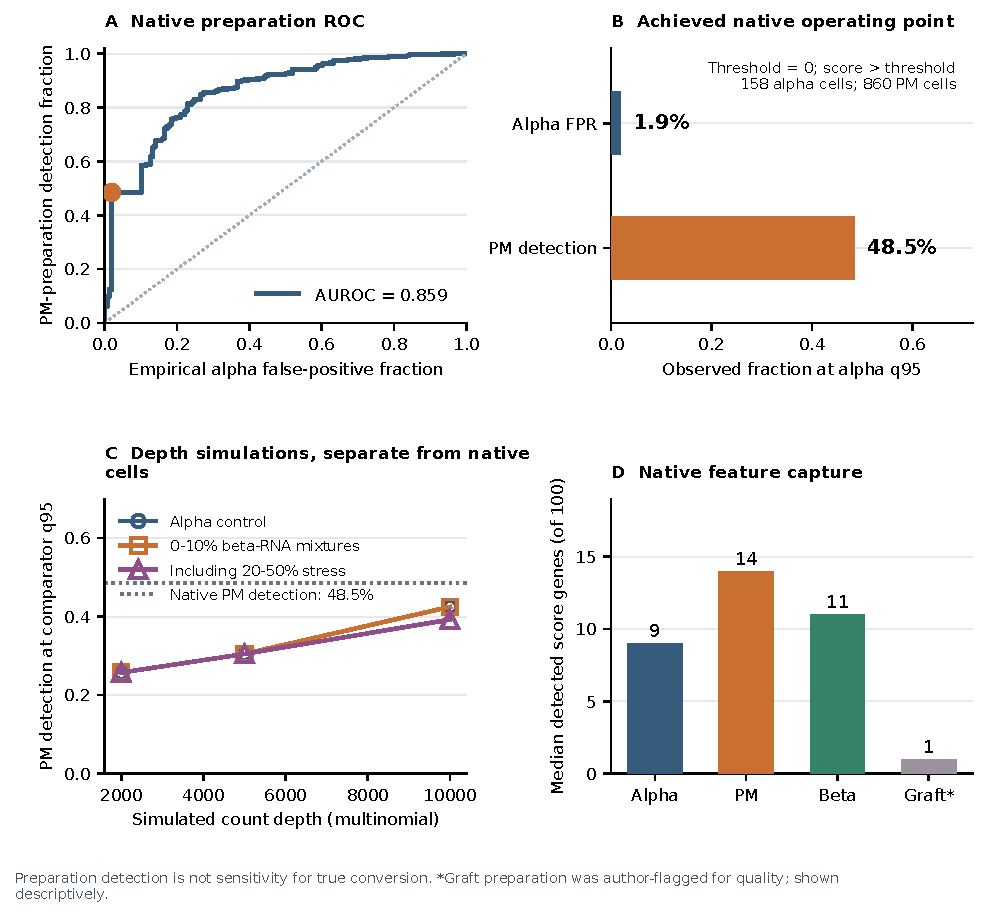
\includegraphics[width=\linewidth]{figures/rev1_figure1_reference.pdf}
\par\small Figure 1. Preparation calibration. A, native PM-versus-alpha ROC. B, detection and achieved false-positive rate at the strict native alpha q95 threshold. C, original multinomial depth simulations, distinct from native baseline and true thinning. D, median detected signature genes. Graft material was author-flagged for quality. Preparation detection is not sensitivity for true conversion.
\end{figure}
\clearpage
\clearpage
\begin{figure}[p]\centering
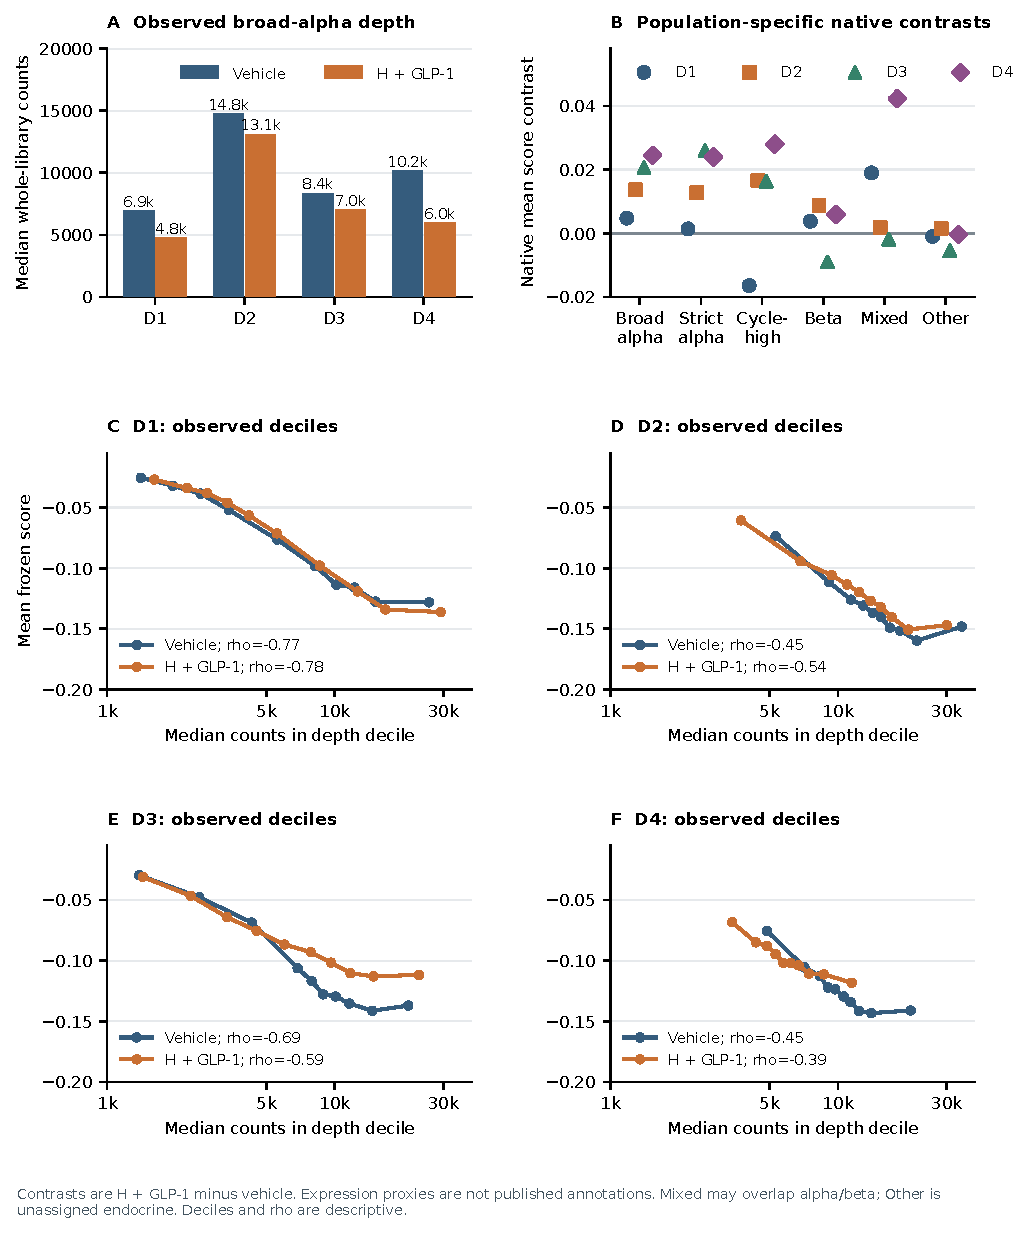
\includegraphics[width=\linewidth]{figures/rev1_figure2_depth_population.pdf}
\par\small Figure 2. Native depth and population context. A, paired broad-alpha median whole-library counts. B, donor contrasts across six expression-proxy populations. C–F, donor-specific depth deciles and descriptive Spearman associations. Mixed-endocrine populations can overlap alpha/beta; other denotes unassigned endocrine cells. None of these proxies encodes ancestry or reproduces published curated annotations.
\end{figure}
\clearpage
\clearpage
\begin{figure}[p]\centering
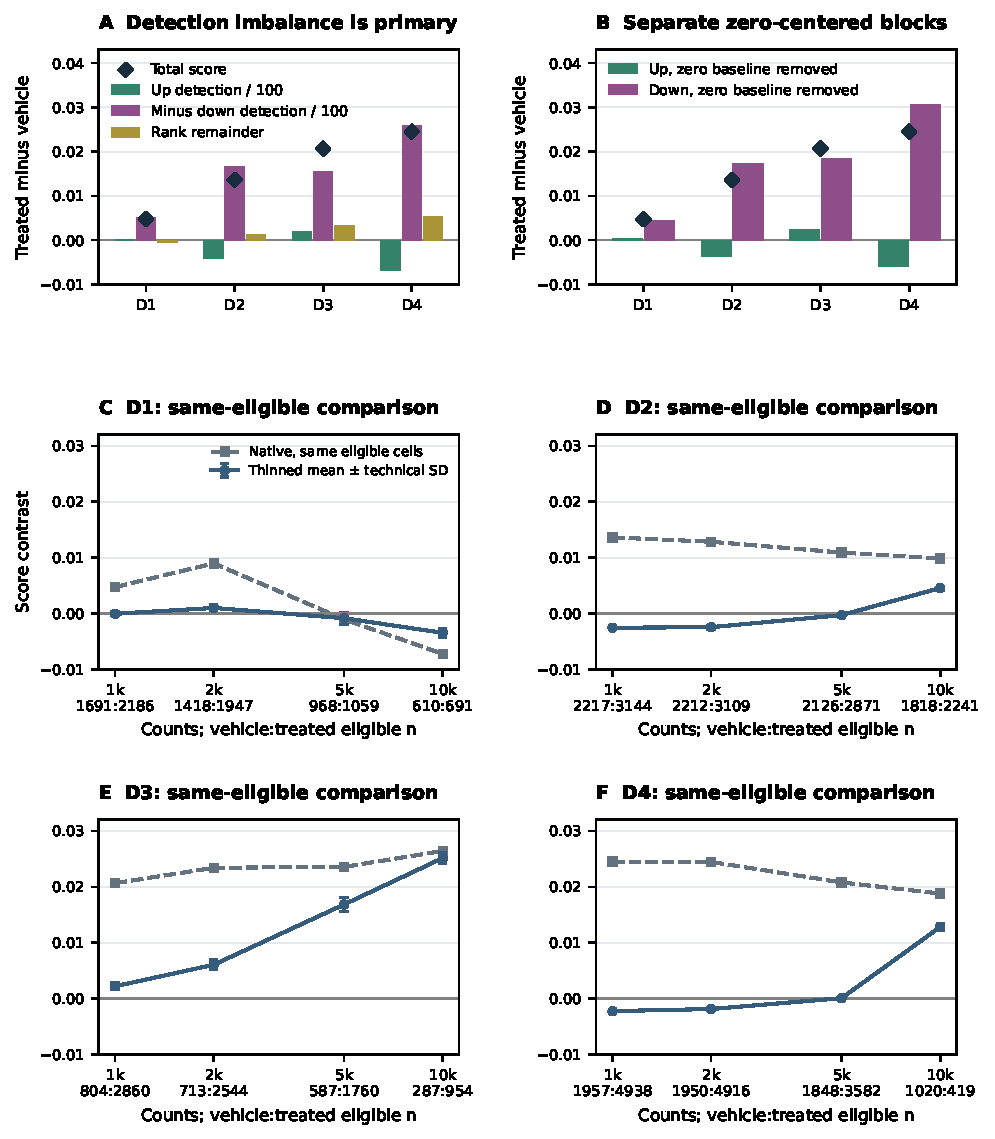
\includegraphics[width=\linewidth]{figures/rev2_mechanism.pdf}
\par\small Figure 3. Detection and sampling. A, up/down occupancy terms and rank remainder. B, separate block contributions after removing their opposite zero-rank baselines. C–F, true-thinning means ± technical SD against native scores on identical eligible cells; labels give vehicle:treated counts. Population masks are fixed, eligibility varies with depth, and no cell is sampled upward.
\end{figure}
\clearpage
\clearpage
\begin{figure}[p]\centering
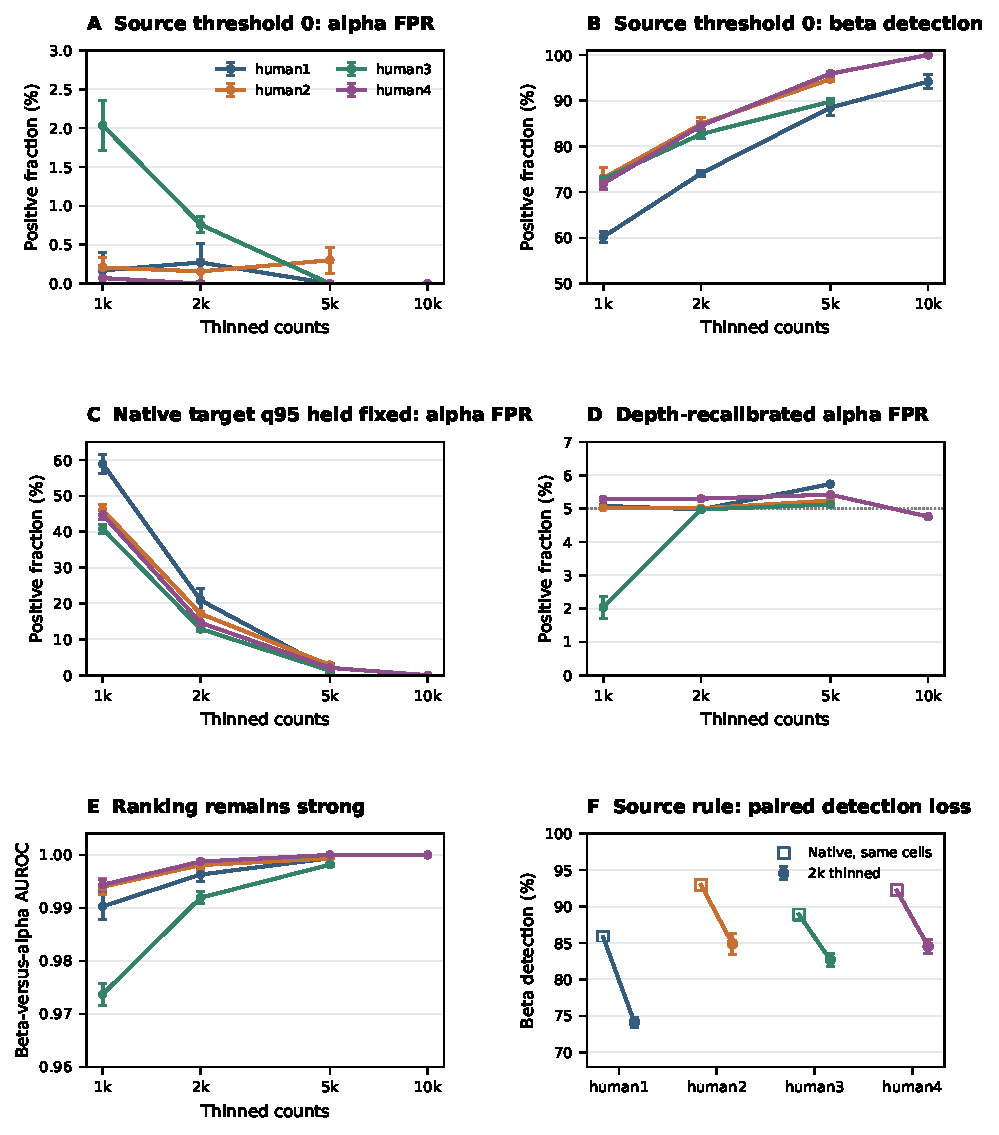
\includegraphics[width=\linewidth]{figures/rev2_threshold_transport.pdf}
\par\small Figure 4. Decision transport under true thinning. A–B, unchanged source threshold. C, each target donor’s native threshold held fixed. D, depth-specific recalibration evaluated on the calibration cells. E, rank AUROC. F, source-rule beta detection at 2,000 counts versus native on identical cells. Error bars are technical SD. Groups below 20 per required state are omitted; eligibility changes across depths.
\end{figure}
\clearpage
\clearpage
\begin{figure}[p]\centering
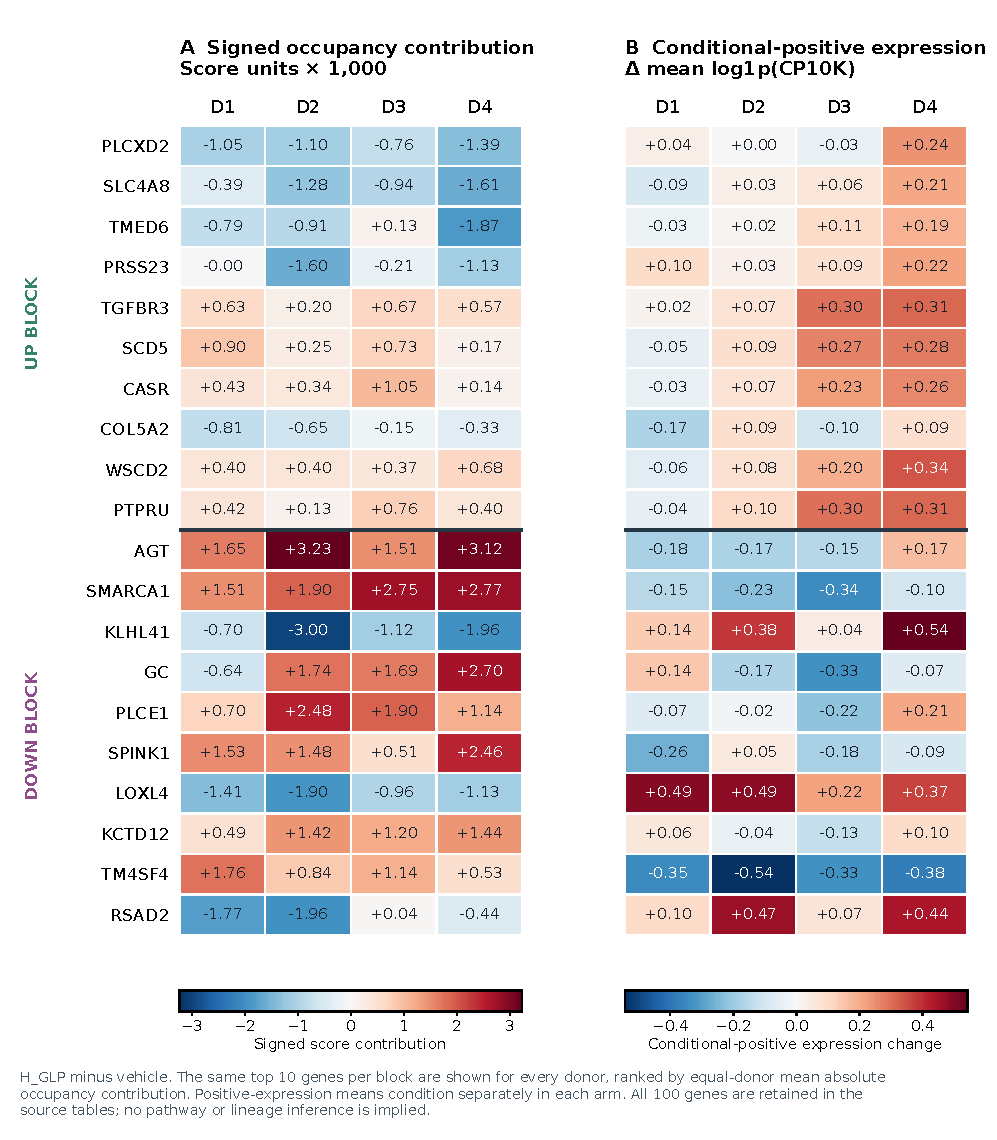
\includegraphics[width=\linewidth]{figures/rev2_gene_drivers.pdf}
\par\small Figure 5. Gene-level interpretation. A, signed occupancy contributions (score units ×1,000). B, changes in mean log1p(CP10K) among cells detecting that gene. The same top ten genes per block use a shared equal-donor absolute-contribution ranking. Positive-cell sets can differ between arms; these are not longitudinal expression changes. All 100 genes remain in the tables.
\end{figure}
\clearpage
\clearpage
\begin{figure}[p]\centering
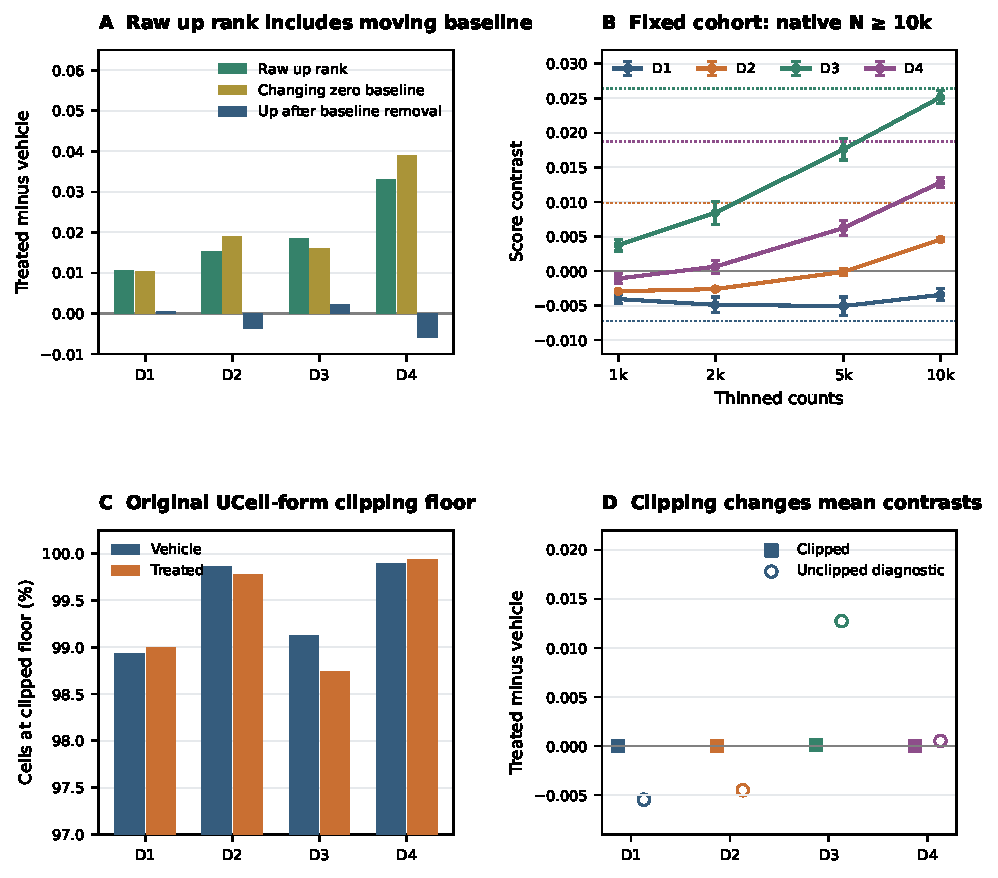
\includegraphics[width=\linewidth]{figures/rev2_supplement_baseline_floor.pdf}
\par\small Figure S1. Explanatory sensitivities. A, raw up-rank contrast, its changing zero baseline, and zero-centered up contrast. B, one N≥10,000 cohort at all depths; dotted lines are native contrasts. C, original UCell-form floor fractions. D, locked clipped and supplementary unclipped contrasts. The high-depth cohort is selected; technical SD describes five existing draws.
\end{figure}
\clearpage
\clearpage
\begin{figure}[p]\centering
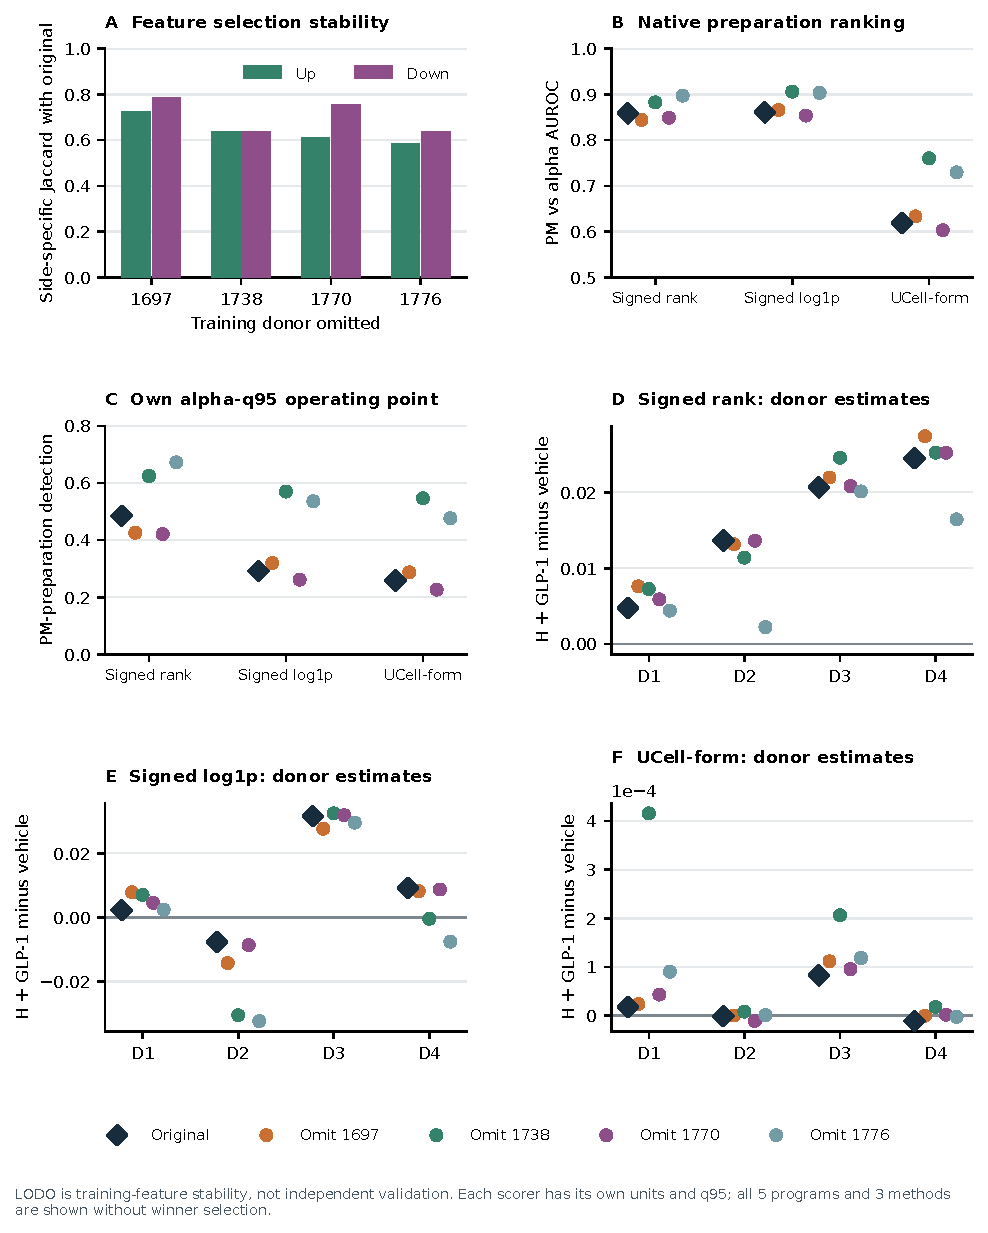
\includegraphics[width=\linewidth]{figures/rev1_figure4_benchmark.pdf}
\par\small Figure S2. All five original feature programs and three locked scorers. A, overlap with original features. B–C, native reference AUROC and preparation detection. D–F, donor contrasts for ranks, log-expression and UCell-form scores. Scorer units differ. Leave-one-donor-out selection assesses feature stability; it is not an unbiased held-out validation.
\end{figure}
\clearpage
\clearpage
\begin{figure}[p]\centering
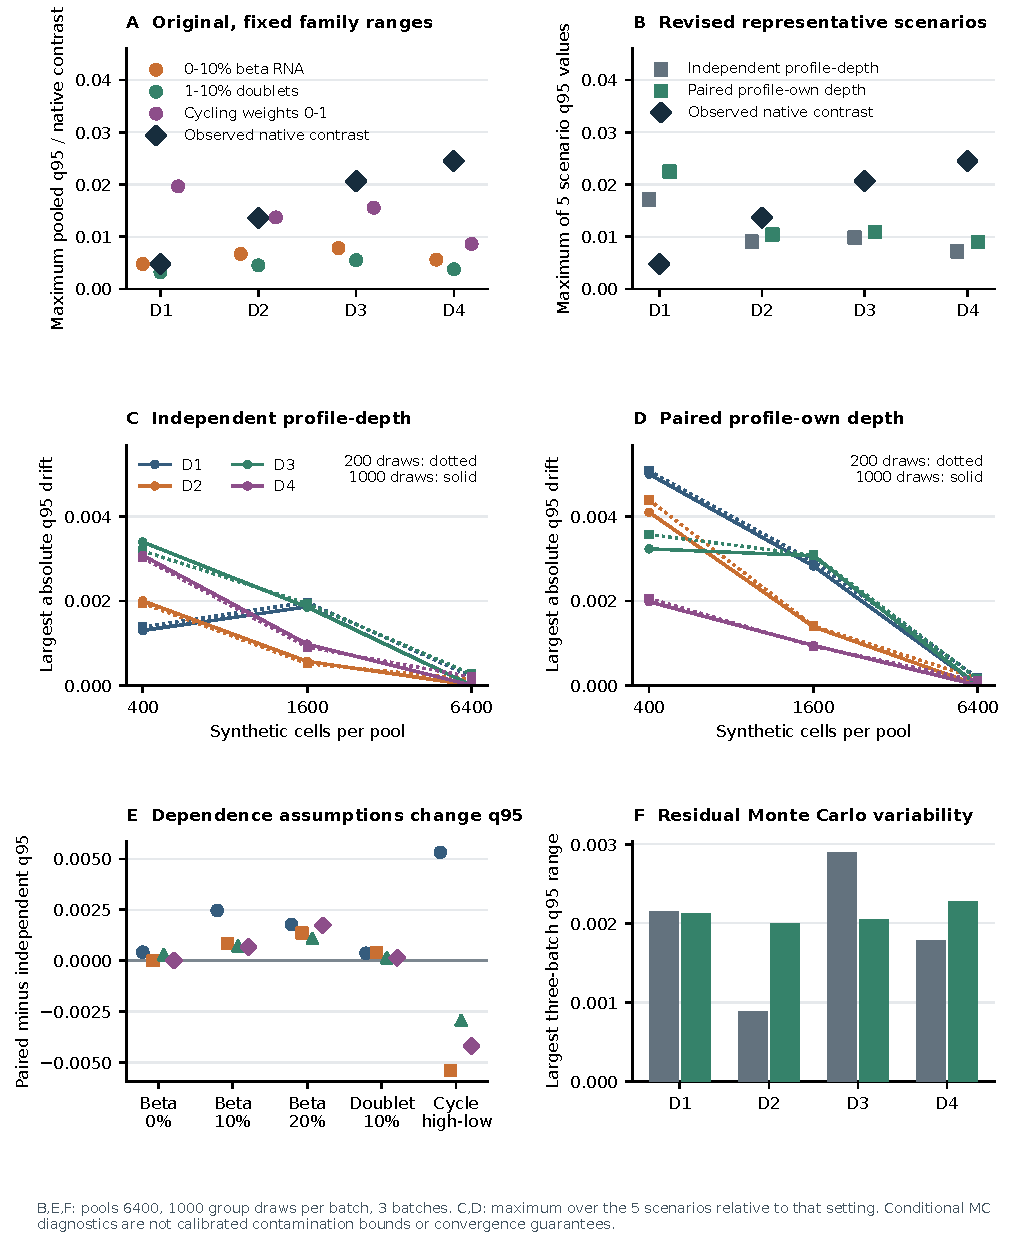
\includegraphics[width=\linewidth]{figures/rev1_supplement_nuisance.pdf}
\par\small Figure S3. Conditional nuisance diagnostics. A, original family maxima (beta RNA through 10\%; Table 3 uses 20\%). B, five revision scenarios at the largest setting. C–D, tail drift with pool size and draws. E, coupling differences. F, three-batch q95 range. Quantiles describe conditional simulation variation; the largest setting does not establish asymptotic convergence or biological confidence coverage.
\end{figure}
\clearpage
\end{document}